\section{86 - MAT - AG 2.1, FA 1.4, FA 2.2, FA 2.4, WS 1.1, WS 1.4 - Human Development Index - Matura 2016/17 2. NT}

\begin{langesbeispiel} \item[0] %PUNKTE DES BEISPIELS
Der Human Development Index ($HDI$) der Vereinten Nationen ist ein Wohlstandsindikator für Länder, der eine Messung des Entwicklungsstandes des jeweiligen Landes ermöglichen sollte.
Der $HDI$ beinhaltet drei dimensionslose Größen (Lebenserwartungsindex ($LEI$), Bildungsindex ($BI$)
und Einkommensindex ($EI$)) und wird mit der Formel $HDI=\sqrt[3]{LEI \cdot BI \cdot EI}$ berechnet.

Dimensionslos bedeutet, dass diese Größen keine Einheiten haben.\leer

Für die Berechnung des Indizes $LEI$ und $EI$ gilt seit 2010:

$LEI=\frac{LE-20}{85-20}$, wobei $LE$ die Lebenserwartung zum Zeitpunkt der Geburt in Jahren beschreibt

$EI=\frac{\ln(B)-\ln(100)}{\ln(75\,000)-\ln(100)}$, wobei $B$ das Bruttonationaleinkommen pro Kopf in US-Dollar (immer zu Jahresbeginn) beschreibt.\leer

Das Entwicklungsprogramm der Vereinten Nationen unterteilt die Länder nach dem Wert des $HDI$ seit 2009 in vier Entwicklungskategorien:


\renewcommand{\arraystretch}{1.5}
\begin{center}
\begin{tabular}{c|c} \hline
\rowcolor{lightgray} Entwicklungskategorie eines Landes & Wert des $HDI$ \\ \hline
$E_1$ & $\leq 0,8$ \\ \hline
$E_2$ & $[0,7; 0,8)$ \\ \hline
$E_3$ & $[0,55; 0,7)$ \\ \hline
$E_4$ & $< 0,55$ \\ \hline
\end{tabular}
\end{center}
\tiny Datenquelle: Deutsche Gesellschaft für die Vereinten
Nationen (Hrsg.): Bericht über die menschliche Entwicklung
2015. Arbeit und menschliche Entwicklung. Berlin:
Berliner Wissenschafts-Verlag 2015, S. 240 \normalsize


Der $HDI$ einer Region in einem bestimmten Jahr ergibt sich aus dem arithmetischen Mittel der $HDI$s der zu dieser Region zählenden Länder. \leer

Die Entwicklung des $HDI$ verschiedener Regionen zwischen 1980 und 2011 ist nachstehend abgebildet.

\begin{center}
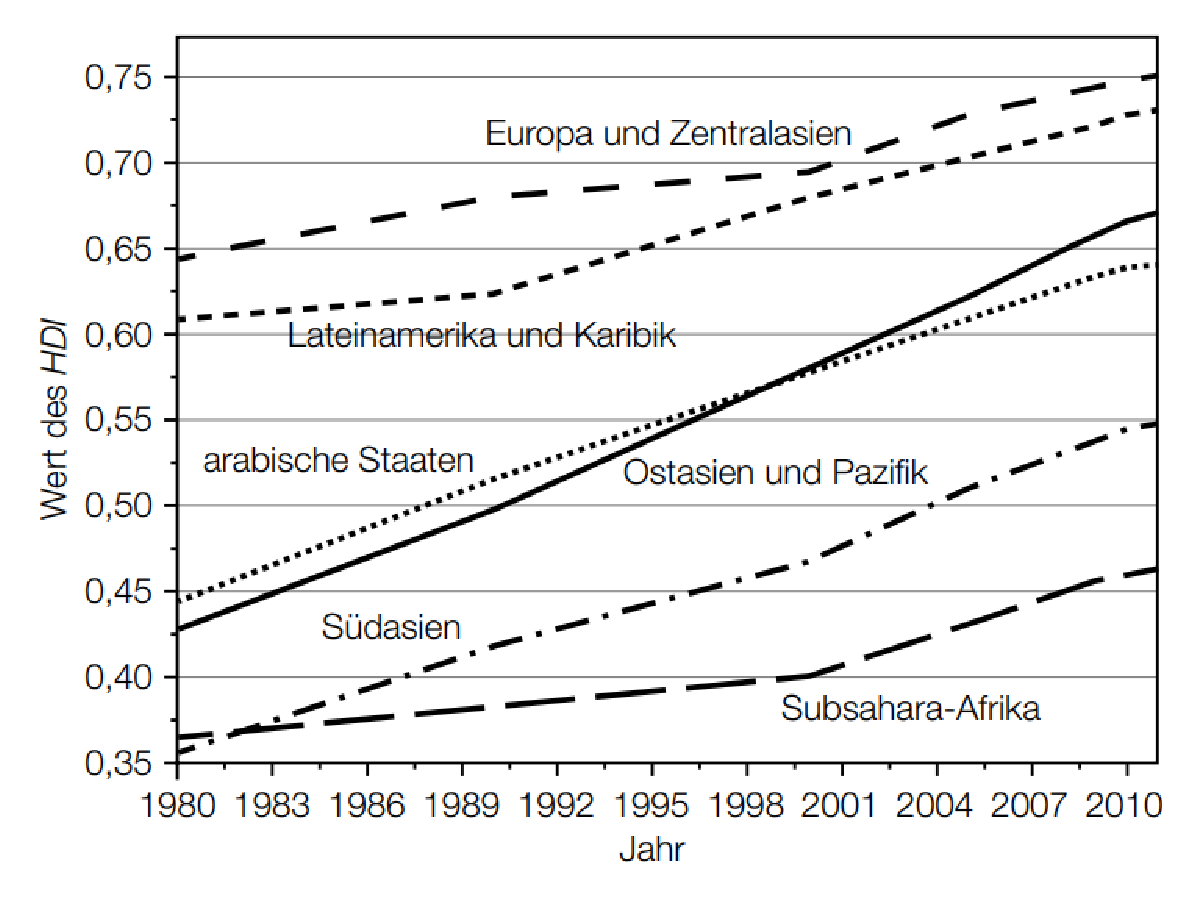
\includegraphics[width=0.7\textwidth]{../Bilder/Bild86-1.eps}
\end{center}
\begin{singlespace}
\tiny Datenquelle: https://de.wikipedia.org/wiki/
Index\_der\_menschlichen\_Entwicklung\#/
media/File:Human-Development-IndexTrends-2011.svg
[08.06.2017]. \normalsize
\end{singlespace}

\subsection{Aufgabenstellung:}

\begin{enumerate}
	\item Für Österreich wurde im Human Development Report für das Jahr 2013 die Lebenserwartung mit $LE = 81,1$ Jahren und der Bildungsindex mit $BI = 0,819$ angegeben. Die nachstehende Abbildung zeigt für die Jahre 2000 bis 2013 (jeweils zu Jahresbeginn) das Bruttonationaleinkommen Österreichs pro Kopf in US-Dollar.
	
\begin{center}
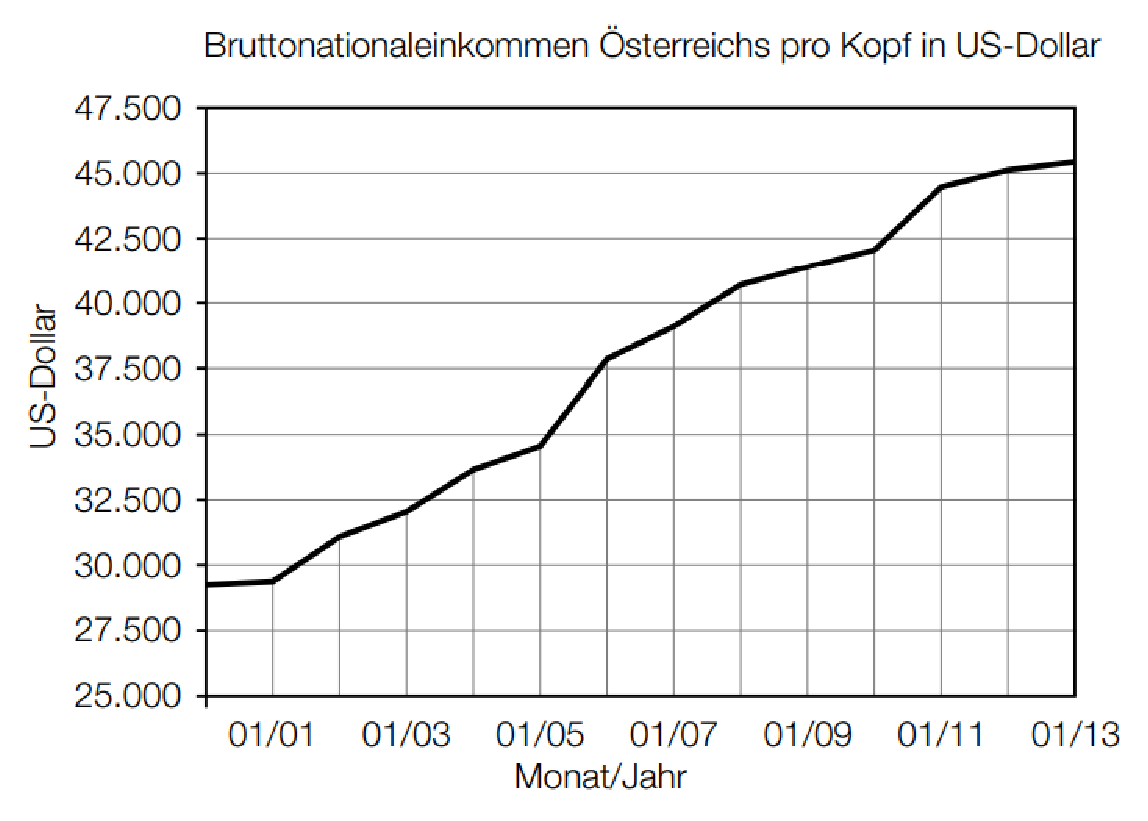
\includegraphics[width=0.6\textwidth]{../Bilder/Bild86-2.eps}
\end{center}	
\tiny Datenquelle: http://www.factfish.com/de/statistik/bruttonationaleinkommen [08.06.2017]. \normalsize

Ermittle für das Jahr 2013 den $HDI$ von Österreich $(=HDI_{2013})$!\leer

Der $HDI$ von Österreich für das Jahr 2013 $(HDI_{2013})$ war um ca. 2,5\,\% größer als der $HDI$ von Österreich für das Jahr 2008 $(HDI_{2008})$. Gib eine Gleichung an, die diesen Zusammenhang beschreibt, und berechne den $HDI_{2008}$!

\item Die jährliche Entwicklung des $HDI$ der Region "`arabische Staaten"' kann im Zeitraum von 1980 bis 2010 näherungsweise durch eine lineare Funktion $H$ mit der Gleichung $H(t) = k \cdot t + d$ mit $k, d \in \mathbb R$ und $t$ in Jahren beschrieben werden, wobei $H(0)$ dem Wert des Jahres 1980 entspricht.\leer

Bestimme die Werte der Parameter $k$ und $d$!\leer

Begründen Sie anhand der entsprechenden Abbildung, in welcher Region/in welchen Regionen die mittlere jährliche Zunahme des $HDI$ im Zeitraum von 1980 bis 2010 am ehesten jener der
Region "`arabische Staaten"' entsprach!

\item \fbox{A} Ermittle aus der entsprechenden Abbildung diejenige Jahreszahl, ab der die Region "`Lateinamerika und Karibik"' die Entwicklungskategorie $E_2$ aufweist!\leer

Gilt ab diesem Zeitpunkt sicher, dass ungefähr die Hälfte der zu dieser Region zählenden Länder
eine Entwicklungskategorie $E_2$ aufweist? Begründe deine Antwort!	
\end{enumerate}

\antwort{
\begin{enumerate}
	\item \subsubsection{Lösungserwartung:}

$LEI=\dfrac{81,1-20}{85-20}=0,94$

$EI\approx \dfrac{\ln(45\,400)-\ln(100)}{\ln(75\,000)-\ln(100)}\approx 0,924$

$HDI_{2013}=\sqrt[3]{0,94\cdot 0,819 \cdot 0,924} \approx 0,893$

$HDI_{2013}=HDI_{2008}\cdot 1,025$

$HDI_{2008}\approx 0,871$

\subsubsection{Lösungsschlüssel}

- Ein Punkt für die richtige Lösung.
Toleranzintervall: $[0,88; 0,91]$
Die Aufgabe ist auch dann als richtig gelöst zu werten, wenn bei korrektem Ansatz das Ergebnis
aufgrund eines Rechenfehlers nicht richtig ist.
- Ein Punkt für eine korrekte Gleichung und die richtige Lösung. Äquivalente Gleichungen sind
als richtig zu werten.
Toleranzintervall: $[0,85; 0,89]$

\item \subsubsection{Lösungserwartung:}

$k=\dfrac{0,64-0,44}{30}=0,006\dot{6}$

$d=0,44$

In der Region "`Südasien"' entsprach die mittlere jährliche Zunahme des HDI im Zeitraum 1980 bis 2010 am ehesten jener der Region "`arabische Staaten"'.

Mögliche Begründung:\\
Die Sekanten durch die Punkte $(1980|0,44)$ und $(2010|0,64)$ sowie $(1980|0,36)$ und $(2010|0,54)$ verlaufen annähernd parallel zueinander. 

\subsubsection{Lösungsschlüssel:}

- Ein Punkt für die Angabe der beiden korrekten Werte.
Toleranzintervall für $k$: $[0,005; 0,01]$
Toleranzintervall für $d$: $[0,43; 0,45]$
- Ein Punkt für die Angabe der Region "`Südasien"' und für eine (sinngemäß) korrekte Begründung.

\item \subsubsection{Lösungserwartung:}

Ab dem Jahr 2004 weist die Region "`Lateinamerika und Karibik"' die Entwicklungskategorie $E_2$
auf.\leer

Nein, es gilt nicht als sicher, dass ab diesem Zeitpunkt ungefähr die Hälfte der zu dieser Region
zählenden Länder die Entwicklungskategorie $E_2$ aufweist.


Mögliche Begründung:
Wenn eine sehr kleine Anzahl an Ländern mit sehr hohen HDI-Werten einer großen Anzahl an
Ländern mit niedrigen $HDI$-Werten $(< 0,7)$ gegenübersteht, kann dennoch das arithmetische
Mittel der $HDI$s größer als $0,7$ sein, ohne dass ungefähr die Hälfte der zu dieser Region zählenden
Länder die Entwicklungskategorie $E_2$ aufweist.

\subsubsection{Lösungsschlüssel:}

- Ein Ausgleichspunkt für die richtige Lösung.
Toleranzintervall: $[2003; 2005]$
- Ein Punkt für eine richtige Antwort und eine korrekte Begründung. Andere korrekte Begründungen
(z.B. anhand sinnvoller Zahlenbeispiele oder mit der Feststellung, dass das arithmetische
Mittel nicht notwendigerweise der Median sein muss) sind ebenfalls als richtig zu
werten.

\end{enumerate}
}

		
\end{langesbeispiel}